\documentclass[10pt, oneside]{article}
\usepackage[utf8]{inputenc}
\usepackage{graphicx} % Required for inserting images
\usepackage{amsmath}
\usepackage{amssymb}
\usepackage[a4paper,left=2.1cm, right=2.1cm, top=2cm, bottom=2cm]{geometry}
\usepackage{verbatim}
\usepackage[english]{babel}
\usepackage{hyperref}
\usepackage{listings}
\usepackage{comment}
\renewcommand{\rmdefault}{cmss}

\lstdefinestyle{mystyle}{	basicstyle=\ttfamily\footnotesize
}

\lstset{style=mystyle}

\title{ROOT}
\author{Pocket reference for 1st year course - BSc Physics, Unibo}
\date{2023}

\begin{document}

\maketitle

\tableofcontents
\newpage
\section{General structure}

ROOT contains \textbf{interpreter} : \textit{Just-In-Time} compilation $\rightarrow$ prompt : special commands (not standard C++ syntax) with \boxed{\texttt{.}}.

Base class \texttt{TObject} $\rightarrow$ \texttt{TNamed} $\rightarrow$ \texttt{TH1} (histograms) $\rightarrow$ \texttt{TH1F, TH1D, THIC, TH1S} according to \textbf{type representing entries} (not the type of data!!)

\section{Basic shell \& prompt commands}
! Possible to use \boxed{Tab}
\begin{itemize}
\item \boxed{\texttt{root}} launch ROOT
\item \boxed{\texttt{.q}} quit
\item \boxed{\texttt{.L <file.C>}} load file (symbols defined in a macro)
\item \boxed{\texttt{.help}} \boxed{\texttt{.?}} full help list
\item \boxed{\texttt{.! <cmd>}} call any shell command <cmd> without leaving ROOT
\item \boxed{\texttt{.files}} shows loaded libraries / sources
\item \boxed{\texttt{.x <macro>}} loads \& runs a macro
\item \boxed{\texttt{.U <file.C>}} unload
\item \boxed{\texttt{.! wslview <image-file>}} (for WSL users) open image with default photo viewer from inside ROOT
\end{itemize}
Run a macro:
\begin{verbatim}
$ [0] .L <name>.C
$ [1] <name>()
\end{verbatim}
Possible to type C++ commands directly in shell: \textbf{';' are unnecessary, object type can be omitted in declarations, possible to access members with obj name instead than pointer}:
\begin{verbatim}
$ [...] TH1F *histo=new TH1F(“histname”,” Titolo”, 100, 0, 10)
$ histname->Draw() // identical to histo->Draw()
\end{verbatim}
\textbf{Note:} \texttt{\#include <iostream>} and \texttt{namespace std;} are implicit!
\paragraph{Use prompt as calculator}
Ordinary operations + embedded library \texttt{TMath}:
\\\texttt{TMath::Abs(...), TMath::Exp(...), TMath::Gaus(...), TMath::Pi(), ...}
\subsection{Recover session history}
Saved in \texttt{\$/home/.root\_hist}

\subsection{\LaTeX{}}
Can be used for labels etc. Same syntax as normal \LaTeX{}
\begin{itemize}
\item \verb^x_{1}^ = $x_1$
\item \verb_x^{1}_ = $x^1$
\end{itemize}
but commands are called with '\texttt{\#}' instead of '\texttt{\textbackslash}'

\section{Macros}
Two types of script
\paragraph{Unnamed script} all code between \{\} + no declaration of classes, functions + no parameters (ok loops)
\paragraph{Named script} like any C++ function + possible to define other functions, classes, use parameters
\\The executed function has the same name of the file (see Basics)

\section{GUI}
\boxed{\texttt{TBrowser b}} opens root files browser. 
\\Double click on an object (e.g. histo) $\rightarrow$ opens new \textbf{TCanvas} and draws it
\subsection*{Handling TCanvas}
if some of the followings not visible, click \textbf{View} and check out
\begin{description}
\item[Editor] single left click on an object in graph $\rightarrow$ edit display parameters (color etc.)
\item[Toolbar] tools to insert text, symbols, etc.
\item[Status bar] shows object pointed by mouse \& mouse position
\item Right click on object $\rightarrow$ contextual menu
\end{description}
\subsubsection*{Contextual menu}
\begin{description}
\item[Rebin] redefine binning
\item[Fit (of FitPanel)] fit a function on data (gaussian, exponential, polynomial etc.) $\rightarrow$ button \texttt{Set Parameters} for chosen distribution
\end{description}
To visualize fit on graph: right click on graph $\rightarrow$ open \texttt{TPaveStats::stats} $\rightarrow$ \texttt{SetOptFit} $\rightarrow$ se to \texttt{111}
\\\texttt{SetOptStat} allows do define other options
\paragraph{Canvas options} Right click on canvas $\rightarrow$ \texttt{SetLogx}, \texttt{SetLogy} for logarithmic scale; \texttt{SetGridx}, \texttt{SetGridy} for grid
\paragraph{Saving file} \texttt{File} $\blacktriangleright$ \texttt{Save} (\texttt{Save As})
\\Saving as \texttt{.C} file (containing the graph as C++ commands) enables to reproduce graph executing macro
\\Saving as \texttt{.root} file $\rightarrow$ saves canvas and all objects, double click on canvas inside .root (opened through TBrowser) to open and manipulate graph

\section{Global variables}
List of useful global pointers.
\begin{description}
\item[\texttt{gROOT}] global info on current session: access to \textbf{every object created during session}
\item[\texttt{gFile}] current root file
\item[\texttt{gStyle}] access functionalities to manage graphic style
\item[\texttt{gRandom}] access random number generator (see PRNG)
\item[\texttt{gPad}] current pad (see Canvas)
\end{description}
\paragraph{Suggestion} at the beginning of a macro, to eliminate copy created by multiple executions of code in a session:
\begin{verbatim}
delete gROOT->FindObject("<name>");
\end{verbatim}
\texttt{gROOT->FindObject("<name>")} used to retrieve every object from gROOT
\subsection*{General styling}
\texttt{gROOT->SetStyle("<style>")} set window style. Can be custom one or chosen between default ones:\\
\texttt{Classic, Plain, Modern, Bold, Video, Pub}

\section{Managing .root files}
\begin{description}
\item[\texttt{TFile *file = new TFile("<name>.root", "RECREATE");}] open file. \texttt{RECREATE} creates new file if name not found, otherwise overwrites existing one. Alternative option: \texttt{"NEW"} (error if already existing!)
\item[\texttt{h->Write();}] write object (pointed by \texttt{h}) on file
\item[\texttt{file->Close();}] close
\end{description}

\section{Histograms}
\textbf{1D}
\begin{verbatim}
TH1F* <pt-name> = new TH1F( "<name>", "<title>", <NxBins>, <xmin>, <xmax>);
// declare new histogram
// range [xmin, xmax] is equally subdivided in N bins

<pt-name>->Fill(<x>); 
// fill histo with variable <x> (e.g. from MC generation or read file, data)

<pt-name>->Fill(<x>, <n>);
// fill histo with n identical occurrences of x

<pt-name>->Draw(); // draw histo
\end{verbatim}
\textbf{2D}
\begin{verbatim}
TH2F* <pt-name> = new TH2F( "<name>","<title>",<NxB>,<xmin>,<xmax>,<NyB>,<ymin>,<ymax>);

<pt-name>->Fill(x,y);
<pt-name>->Draw();

<pt-name>->ProjectionX(); // returns TH1F of projection w.r.t. x
<pt-name>->ProjectionY();
\end{verbatim}
\textbf{3D}
\begin{verbatim}
TH3F* <pt-name> = new TH2F( "<name>","<title>",<Nx>,<xmn>,<xmx>,<Ny>,<ymn>,<ymx>,<Nz>,<zmn>,<zmx>);
\end{verbatim}
\textbf{N-D}
\begin{verbatim}
THnSparse* pt = new THSparse( "<name>", "<title>", <Ndims>, <xmin>, <xmax>, <chuncksize>); 
// min and max same for all dimensions
\end{verbatim}

\subsection{Overlap histos}
\begin{verbatim}
// declare and initialize two histos, with pointers h1, h2
h1->Draw();
h2->Draw("same"); // or h2->Draw("SameHist");
\end{verbatim}

\subsection{Histo Draw options}
\begin{description}
\item[\texttt{"E"}] show error bars
\item[\texttt{"hist"}] show only histogram
\item[\texttt{"lego"}] lego plot
\item[\texttt{"cont"}] contour lines (linee di livello)
\item[\texttt{"Surf"}] surface
\item[\texttt{"P"}] draw marker (except empty bins)
\item[\texttt{"AXIS"}] draw only axis
\item[\texttt{"AXIG"}] draw only grid (if requested)
\item[\texttt{"FUNC"}]	When histo has fitted function, draw the fit result only.
\item[\texttt{"TEXT"}]	Draw bin contents as text (format set via 
\texttt{gStyle->SetPaintTextFormat}).
\item[\texttt{"X+"}]	The X-axis is drawn on the top side of the plot.
\item[\texttt{"Y+"}]	The Y-axis is drawn on the right side of the plot.
\item[\texttt{"MIN0"}] Set minimum value for the Y axis to $0$, equivalent to \texttt{gStyle->SetHistMinimumZero()}.
\end{description}
\boxed{\textbf{OPTIONS ARE NOT CASE SENSITIVE}}
\\~\\They can also be concatenated without spaces \& commas: \texttt{"opt1 opt2"}
\subsection{Cosmetics for histos}
\begin{description}
\item[\texttt{h1->SetMarkerStyle(<code>);}] set style, see $\uparrow$ for codes:
\begin{figure}[h!]
\centering
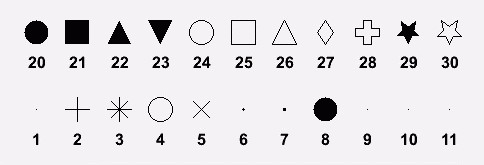
\includegraphics[scale=0.6]{shape.jpg}
\end{figure}
\item[\texttt{h1->GetXaxis()->SetTitle("<title>")}] change axis title, same for y with \texttt{GetYaxis()}
\item[\texttt{SetFillColor(<color>)}] see after for codes
\item[\texttt{SetFillColorAlpha(<color>, <transparency ratio>)}] allows to manipulate opacity, \\e.g. \texttt{(kBlue, 0.35)}
\item[\texttt{SetLineColor(<color>)} or  \texttt{SetLineColorAlpha(<color>, <transp>)}]
\item[\texttt{SetLineStyle(<code>)}] see below
\item[\texttt{SetLineWidth(<width>)}] see below
\end{description}
\begin{figure}[h!]
\centering
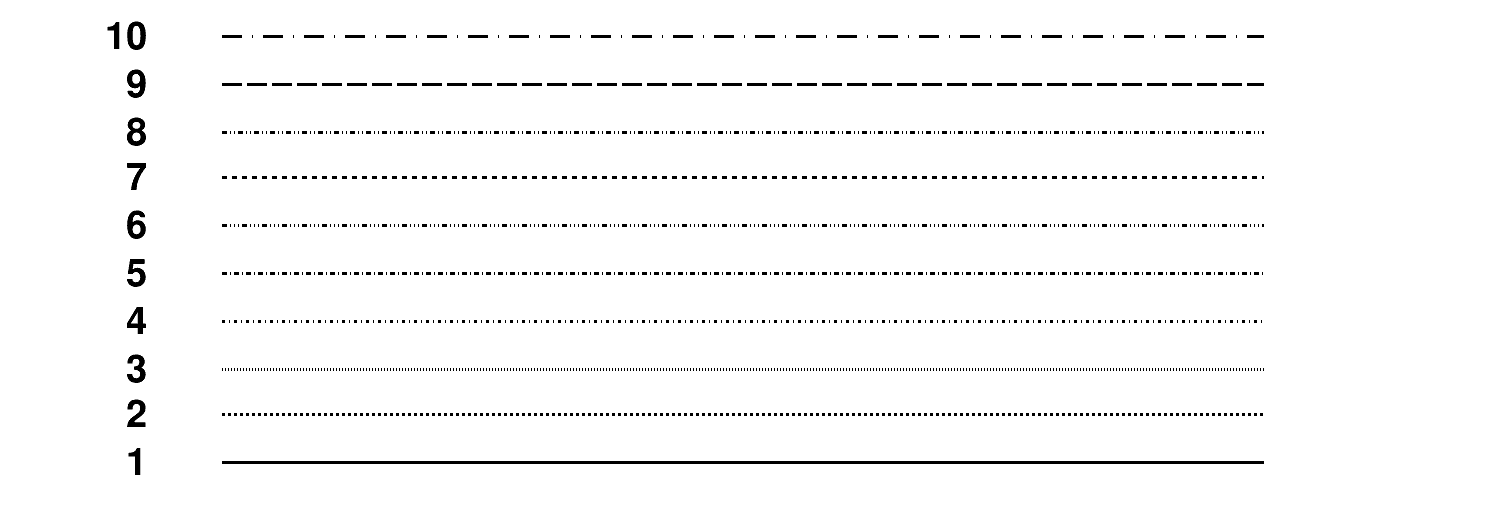
\includegraphics[scale=0.22]{linestyle.png}
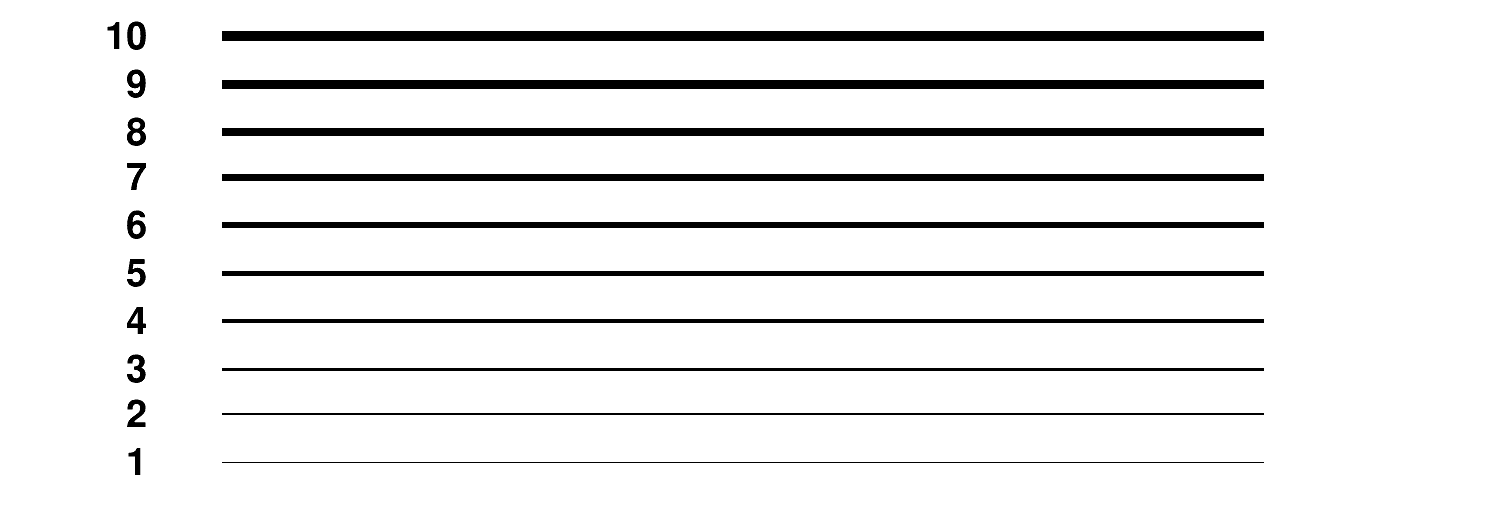
\includegraphics[scale=0.2]{linewidth.png}
\end{figure}

\subsection{Other member functions for histos}
\begin{description}
\item[\texttt{GetMean()}] mean
\item[\texttt{GerRMS()} \texttt{GetStdDev()}]root of variance / SD
\item[\texttt{GetMaximum()}] maximum bin content
\item[\texttt{GetMaximumBin()}] location of maximum ($\neq$ former)
\item[\texttt{GetBinCenter( <bin\_number> )}] center of bin
\item[\texttt{GetBinContent( <bin\_number> )}] content of bin
\item[\texttt{GetBinError( <bin\_number> )}]
\item[\texttt{SetBinContent( <bin\_number>, <value> )}]
\item[\texttt{SetBinError( <bin\_number>, <value> )}]
\end{description}
\textbf{Note:} for out-of-range entries:
\\\texttt{GetBinContent(0)} returns number of \textbf{underflow}
\\\texttt{GetBinContent(<Nbins + 1>)} return number of \textbf{overflow}
\begin{description}
\item[\texttt{GetEntries()}] total entries (includes under/overflows)
\item[\texttt{Integral( <bin\_index1>, <bin\_index2> )}] integral on specified range
\item[\texttt{Integral()}] total integral
\item[\texttt{GetIntegral()}] array of cumulative entries
\item[\texttt{GetMeanError()}] error on mean estimate
\item[\texttt{GetRMSError()} \texttt{GetStdDevError()}] error on RMS estimate
\end{description}

\subsection{Operations on histos}
Form homologue histograms (\textbf{same range and number of bins}): overloads for \textbf{istances}, \textbf{NOT POINTERS}:
\begin{verbatim}
TH1F h1;
TH1F h2 = 3*h1;
TH1F h3 = h1+h2;
\end{verbatim}
Otherwise through methods:
\begin{verbatim}
h->Add(<pt1>, <pt2>, <n1>, <n2>); // sum stored in *h, *h = n1*h1+n2*h2
h->Multiply(3);
h->Divide(<pt1>, <pt2>, <n1>, <n2>); // analogous to sum
\end{verbatim}

\subsection{Filling a histo from ascii file}
\begin{verbatim}
TH1F *h1 = new TH1F("h1","Tempi di Caduta",8,-0.5,15.5); 

ifstream in;
in.open("maxwell.dat");
Float_t x,y;
while (1) { // always true condition: iterates until break called
   in >> x >> y;
   if(!in.good()) break;
   h1->Fill(y);
}
in.close();
\end{verbatim}


\section{Graphs}
Two classes: \textbf{\texttt{TGraph}} (series of N X-Y couples), \textbf{\texttt{TGraphErrors}} (derived from former, includes also errors on both X and Y)
\paragraph{TGraph Constructors} Derived class!
\begin{description}
\item[\texttt{TGraph (Int\_t n, const Double\_t *x, const Double\_t *y)
}] n couples, \texttt{x} and \texttt{y} are \textbf{arrays}!
\item[\texttt{TGraph (const char *filename, const char *format="\%lg \%lg", 
Option\_t *option="")}] input file \textbf{must contain 2 separate columns of values} (divided by blank delimiter) 
\\Default format: \texttt{"\%lg \%lg"} (2 double), to skip columns: \texttt{\%lg \%*lg \%lg"}
\\Additional options to interpret different delimiters: can be explicitly specified in option argument ( \texttt{option = "<symbol>"} )
\end{description}
\paragraph{TGraphErrors Constructors}
\begin{description}
\item[\texttt{TGraphErrors (Int\_t n, const Double\_t *x, const Double\_t *y, const Double\_t*ex=0, const Double\_t *ey=0)}] analogous to TGraph, \texttt{ex}, \texttt{ey} = arrays of errors (for negligible/null uncertainty: substitute with \texttt{0})
\item[\texttt{TGraphErrors (const char *filename, const char *format="\%lg \%lg \%lg \%lg", Option\_t *option="")}] input file \textbf{must contain at least 3 columns}. If there are 4 (or more, only first 4 read): X, Y, EX, EY. If only 3: X,Y,EY.
\end{description}
\boxed{\textbf{COMMA FOR DECIMALS MUST BE REPLACED WITH DOT}}

\subsection{Graph member functions}
(\texttt{graph} here is the pointer) \, | \, inherited by \texttt{TGraphErrors} !\\
\textbf{Cosmetics:}
\begin{description}
\item[\texttt{graph->SetTitle("<title>")}]
\item[\texttt{graph->SetMarkerStyle(kOpenCircle)}] (here \texttt{kOpenCircle} is default code)
\item[\texttt{graph->SetMarkerColor(kBlue)}] (\texttt{kBlue} also default)
\item[\texttt{graph->SetLineColor(kBlue)}] ...
\end{description}
\textbf{Statistical properties:}
\begin{description}
\item[\texttt{graph->GetCorrelationFactor()}]
\item[\texttt{graph->GetCovariance()}]
\item[\texttt{graph->GetPoint(<i>,<x>,<y>)}] returns \texttt{i}-th point
\item[\texttt{graph->GetX() / graph->GetY()}] returns pointer to array of x / y values
\item[\texttt{graph->GetN}]
\item[\texttt{graph->Integral()}]
\end{description}
\textbf{Other:}
\begin{description}
\item[\texttt{graph->AddPoint(<x>,<y>)}]
\item[\texttt{graph->SetPoint(<i>, <x>, <y>)}]
\item[\texttt{graph->GetXaxis()}] pointer to X axis
\item[\texttt{graph->GetYaxis()}] pointer to Y axis
\item[\texttt{graph->SetMinimum(<double>)}] set minimum on Y
\item[\texttt{graph->SetMaximum(<double>)}] set maximum on Y
\end{description}

\subsection{Color reference}
\begin{figure}[h!]
\centering
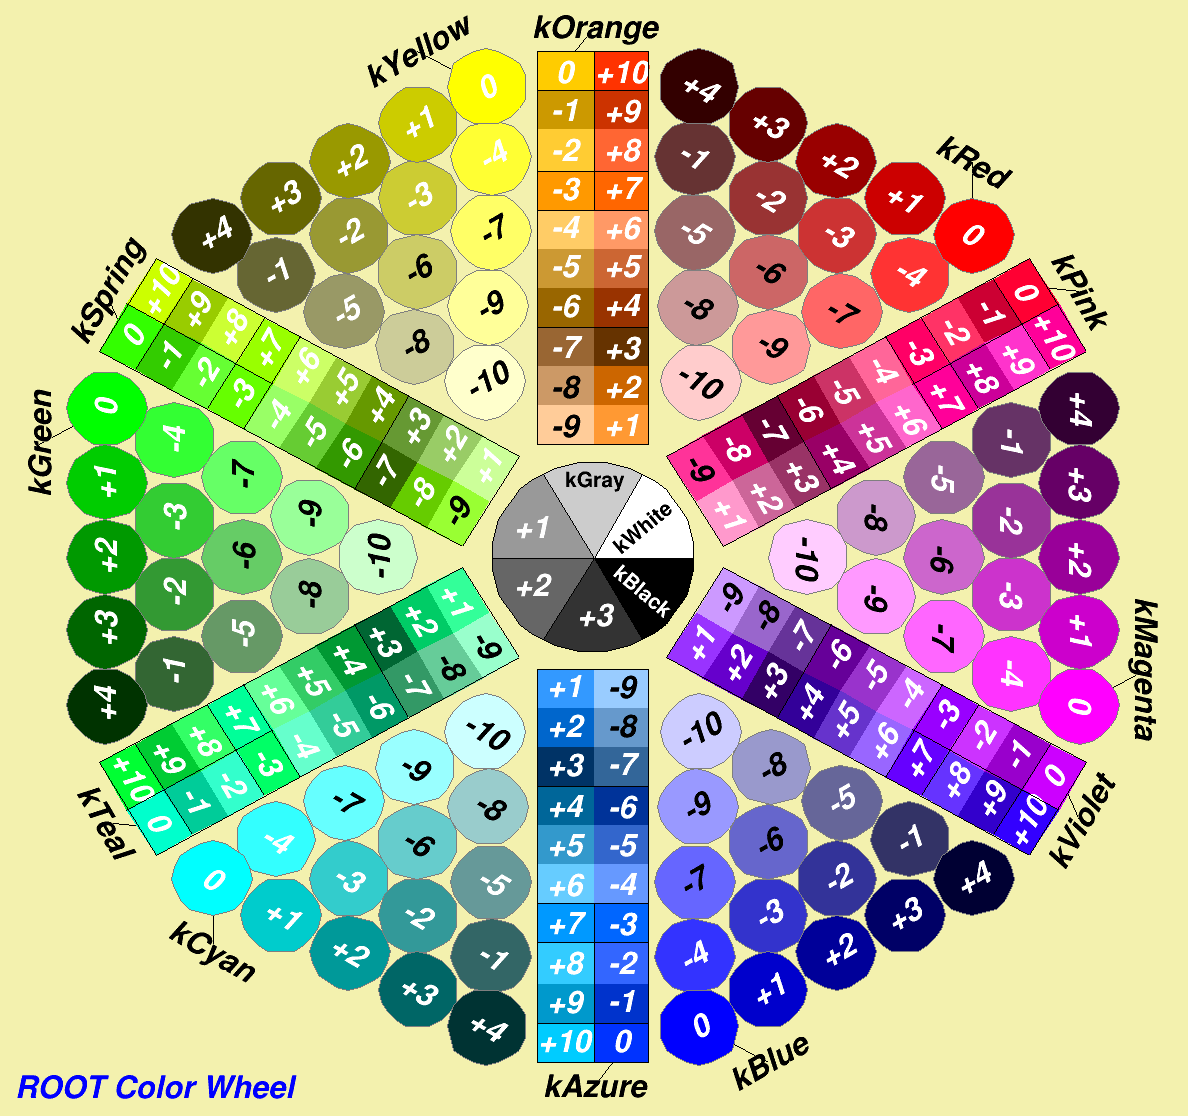
\includegraphics[scale=0.25]{maxres.png}
\end{figure}
~\\
\subsection{Drawing TGraph}
\begin{description}
\item[\texttt{graph->Draw(<options>)}]
\item[\texttt{"A"}] draws axis
\item[\texttt{"P"}] draws points markers (the current one set)
\item[\texttt{"E"}] draws error bars
\item[\texttt{"AI"}] draws invisible axis (no labels)
\item[\texttt{*}] draws star at each point (alternative to $P$)
\item[\texttt{C}] draws a smooth curve connecting points
\item[\texttt{X+}] X axis drawn on the top side
\item[\texttt{Y+}] Y axis drawn on the right side
\item[\texttt{RX}] reverse the X axis
\item[\texttt{RY}] reverse the Y axis
\end{description}
\subsection{Drawing TGraphErrors}
Along with previous options, some specific ones:
\begin{description}
\item[\texttt{Z}] do \textbf{not} draw horizontal and vertical lines at the end of error bars
\item[\texttt{>}] draw arrow at the end
\item[\texttt{|>}] filled arrow
\item[\texttt{X}] do \textbf{not} draw error bars
\item[\texttt{||}] draw only lines at the end of bars, \textbf{not} bars themselves
\item[\texttt{0}] force error bars drawing also for points outside visible range along Y (by default they're not drawn)
\item[\texttt{2}] draw error rectangles
\item[\texttt{3}] filled area through the end points
\item[\texttt{4}] smoothed filled area
\item[\texttt{5}] like \texttt{2}, but countour lines are drawn.

\end{description}
\subsection{Additional styling}
\begin{description}
\item[\texttt{gStyle->SetErrorX(<dx>)}] if set to $0$ removes error along x
\item[\texttt{gStyle->SetEndErrorSize(<n\_px>)}] size of line at the end of error bars. Default = $1$.
\end{description}

\subsection{Fit}
The following syntax is valid both for histos and graphs.
\begin{description}
\item[\texttt{Fit( "<name>", <option>, <graphic\_opt>, <xmin>, <xmax>)}] where \texttt{name} is one of the defaults: \texttt{gaus, gausn} (normalized), \texttt{landau, landaun, expo, pol1, pol2, ..., pol9} (polynomial of degree $n$), \texttt{chebyshev1, chebyshev2, ..., chebyshev9}\\
To print list of avaiable functions: \begin{verbatim}
TF1::InitStandardFunctions(); // not needed if `gROOT->GetFunction` is called before
gROOT->GetListOfFunctions()->ls()
\end{verbatim}
\texttt{name} can also be a formula accepted by the linear fitter with the operator \texttt{++}\\
(e.g. \texttt{x++sin(x)}, for fitting \texttt{[0]*x+[1]*sin(x)})
\item[\texttt{Fit( TF1* f1, <option>, <graphi\_opt> , <xmin>, <xmax> )}] with previously defined function (see after)
\end{description}
\texttt{graphic\_opt} is analogous to the one for \texttt{Draw}, whereas \texttt{option} can contain one (or more) of the following:
\begin{description}
\item[FOR HISTOS ONLY]
\item[\texttt{L}] use logarithmic likehood method (instead of default Chi square)

\item[\texttt{WIDTH}] scales histogram bin content by bin width (useful for variable bins)
\item[\texttt{MULTITHREAD}] forces employment of multithreading whenever possible
\item[FOR GRAPHS ONLY]
\item[\texttt{W}] ignore point errors when fitting TGraphErrors
\item[FOR BOTH HISTOS AND GRAPHS]
\item[\texttt{R}] use fitting range specified in the function range (default is histo's)
\item[\texttt{C}] in case of linear fit, disables calculation of Chi square (saves CPU time)
\item[\texttt{Q}] quiet mode: print minimum data
\item[\texttt{V}] verbose mode: print everything
\item[\texttt{S}] stores full fit result and returns a \texttt{TFitResultPtr} for access
\end{description}

\begin{description}
\item[\texttt{TF1* fitFunc = <pt>->GetFunction("f1")}] recover fit function from histo (analogous for graph)
\item[\texttt{fitFunc->GetChiSquare()}]
\item[\texttt{fitFunc->GetParameter(<i>)}] \texttt{i}-th parameter value
\item[\texttt{fitFunc->GetParError(<i>)}] error on \texttt{i}-th parameter
\end{description}

\subsubsection{Statistics \& fit parameters}
\texttt{gStyle->SetOptStat(<ksiourmen>)} choose statistics parameters to be displayed \\
(each mode with a value - default \textbf{0} if omitted):
\begin{itemize}
\item[\texttt{k}] \textbf{1} = print kurtosis, \textbf{2} = print kurtosis + k. error
\item[\texttt{s}] \textbf{1} = print skewness, \textbf{2} = print skewness + s. error
\item[\texttt{i}] \textbf{1} =print integral of bins, \textbf{2} = print integral of bins with option 
\item[\texttt{o}] \textbf{1} = print number of overflows
\item[\texttt{u}] \textbf{1} = print number of underflows
\item[\texttt{r}] \textbf{1} = print SD \textbf{2} = print SD + SD error \footnote{Actually \texttt{r} stands for Root Mean Square, defined according to 
\[x_{RMS} = \sqrt{\frac{1}{n} \sum x_i^2}\]
} 
\item[\texttt{m}] \textbf{1} = print mean \textbf{2} = print mean + mean error
\item[\texttt{e}] \textbf{1} = print number of entries
\item[\texttt{n}] \textbf{1} = print histogram name 
\end{itemize}
\textbf{STARTS FROM THE END:} 
\begin{verbatim}
gStyle->SetOptStat(11); // only name + entries
gStyle->SetOptStat(1101); // name, mean, RMS
\end{verbatim}
\texttt{gStyle->SetOptFit(<pcev>)} analogous for fit parameters:
\begin{itemize}
\item[\texttt{p}] \textbf{1} = print Probability
\item[\texttt{c}] \textbf{1} = print Chisquare / Number of d.o.f.
\item[\texttt{e}] \textbf{1} = print errors
\item[\texttt{v}] \textbf{1} = print name/values of parameters (only non-fixed) \textbf{2} = print name/value of \textit{all} parameters
\end{itemize}
\texttt{gStyle->SetOptFit(1)} is \textbf{equivalent} to \texttt{gStyle->SetOptFit(111)} (!)

\section{Functions}
In 1 variable (x): class \textbf{TF1}. User-defined function (and function objects, lambda) or built-in function objects $\rightarrow$ \textbf{TFormula}
\\For more dimensions (variables) \textbf{TF2, TF3}.
\begin{description}
\item[\texttt{TF1 *f1 = new TF1("f1", "sin(x)/x",<xmin>,<xmax>)}]
\item[\texttt{TF1 *f2 = new TF1("f2", "f1 * 2",0,10)}] previously defined functions can be used in definition of new ones
\item[\texttt{TF1 *f3 = new TF1("f3","[0]*x*sin([1]*x)",-3,3)}] possible to use parameters: to \textbf{initialize} them, \\\texttt{f3->SetParameter(<value0>, <value1>)}
\end{description}
\begin{verbatim}
Double_t MyFunction(Double_t *x, Double_t *par){ 
    Float_t xx = x[0];
    Double_t val = TMath::Abs(par[0]*sin(par[1]*xx)/xx); 
    return val;
}
\end{verbatim}
\textbf{Note:} important to follow this signature!
\begin{description}
\item[\texttt{TF1 *f4 = new TF1("f4",MyFunction,0,10,2);}] {}\,\\
last constructor parameter is \textbf{number of parameters in MyFunction}
\end{description}
\paragraph{Cosmetics}
\begin{description}
\item[\texttt{f1->SetLineColor(kRed)}]
\item[\texttt{f1->SetLineStyle(2)}] 2 = dashed, 3 = dotted, 4 = dasheddotted
\end{description}
\paragraph{Member functions:}
\begin{description}
\item[\texttt{f1->Eval(<x\_value>)}] evaluate on a point
\item[\texttt{f1->Integral(<a>, <b>)}] compute $\displaystyle \int_a^b f1$
\item[\texttt{f1->SetMaximum(<value>)}] set maximum for Y axis
\item[\texttt{f1->SetMinimum(<value>)}] minimum for Y axis
\item[\texttt{f1->SetRange( <x\_min> , <x\_max> )}] set interval for indipendent variable to \texttt{\big[x\_min,x\_max\big]}
\end{description}

\section{Legend}
\begin{verbatim}
TLegend *leg = new TLegend(<x1>,<y1>,<x2>,<y2>,“ <title> ");
\end{verbatim}
$(x1,y2)$ = bottom left corner, $(x2,y2)$ = upper right corner \textbf{in normalized coordinates}, so $1$ = \textbf{pad} height / width
\[x = \frac{absolute \enspace horizontal \enspace position}{screen \enspace width} \qquad y = \frac{absolute \enspace vertical \enspace position}{screen \enspace height}\]
$x$ goes from left to right, $y$ from bottom to top\\
Careful when using more pads (see\textbf{ Canvas syntax})
\begin{verbatim}
leg->AddEntry(graph,"Punti sperimentali"); 
leg->AddEntry(f,"Fit Lineare"); 
leg->AddEntry(<object>,"<description>");
leg->AddEntry(<object>,"<description>", "<option>"); // alternative syntax
\end{verbatim}
Possible options:
\begin{verbatim}
leg->Draw("Same"); 
leg->SetTextAlign(31); // right
\end{verbatim}
\paragraph{Cosmetics (\texttt{gStyle} member functions)}
\begin{verbatim}
gStyle->SetLegendBorderSize(<n>);
gStyle->SetLegendFillColor(<color>);
gStyle->SetLegendFont(<n>); // see below
gStyle->SetLegendTextSize(<size>); // see below
\end{verbatim}
\begin{center}
\textbf{font code (\texttt{<n>}) = 10 $\times$ font number + precision}
\end{center}
Example of fonts with precision $= 2$:
\begin{figure}[h!]
\centering
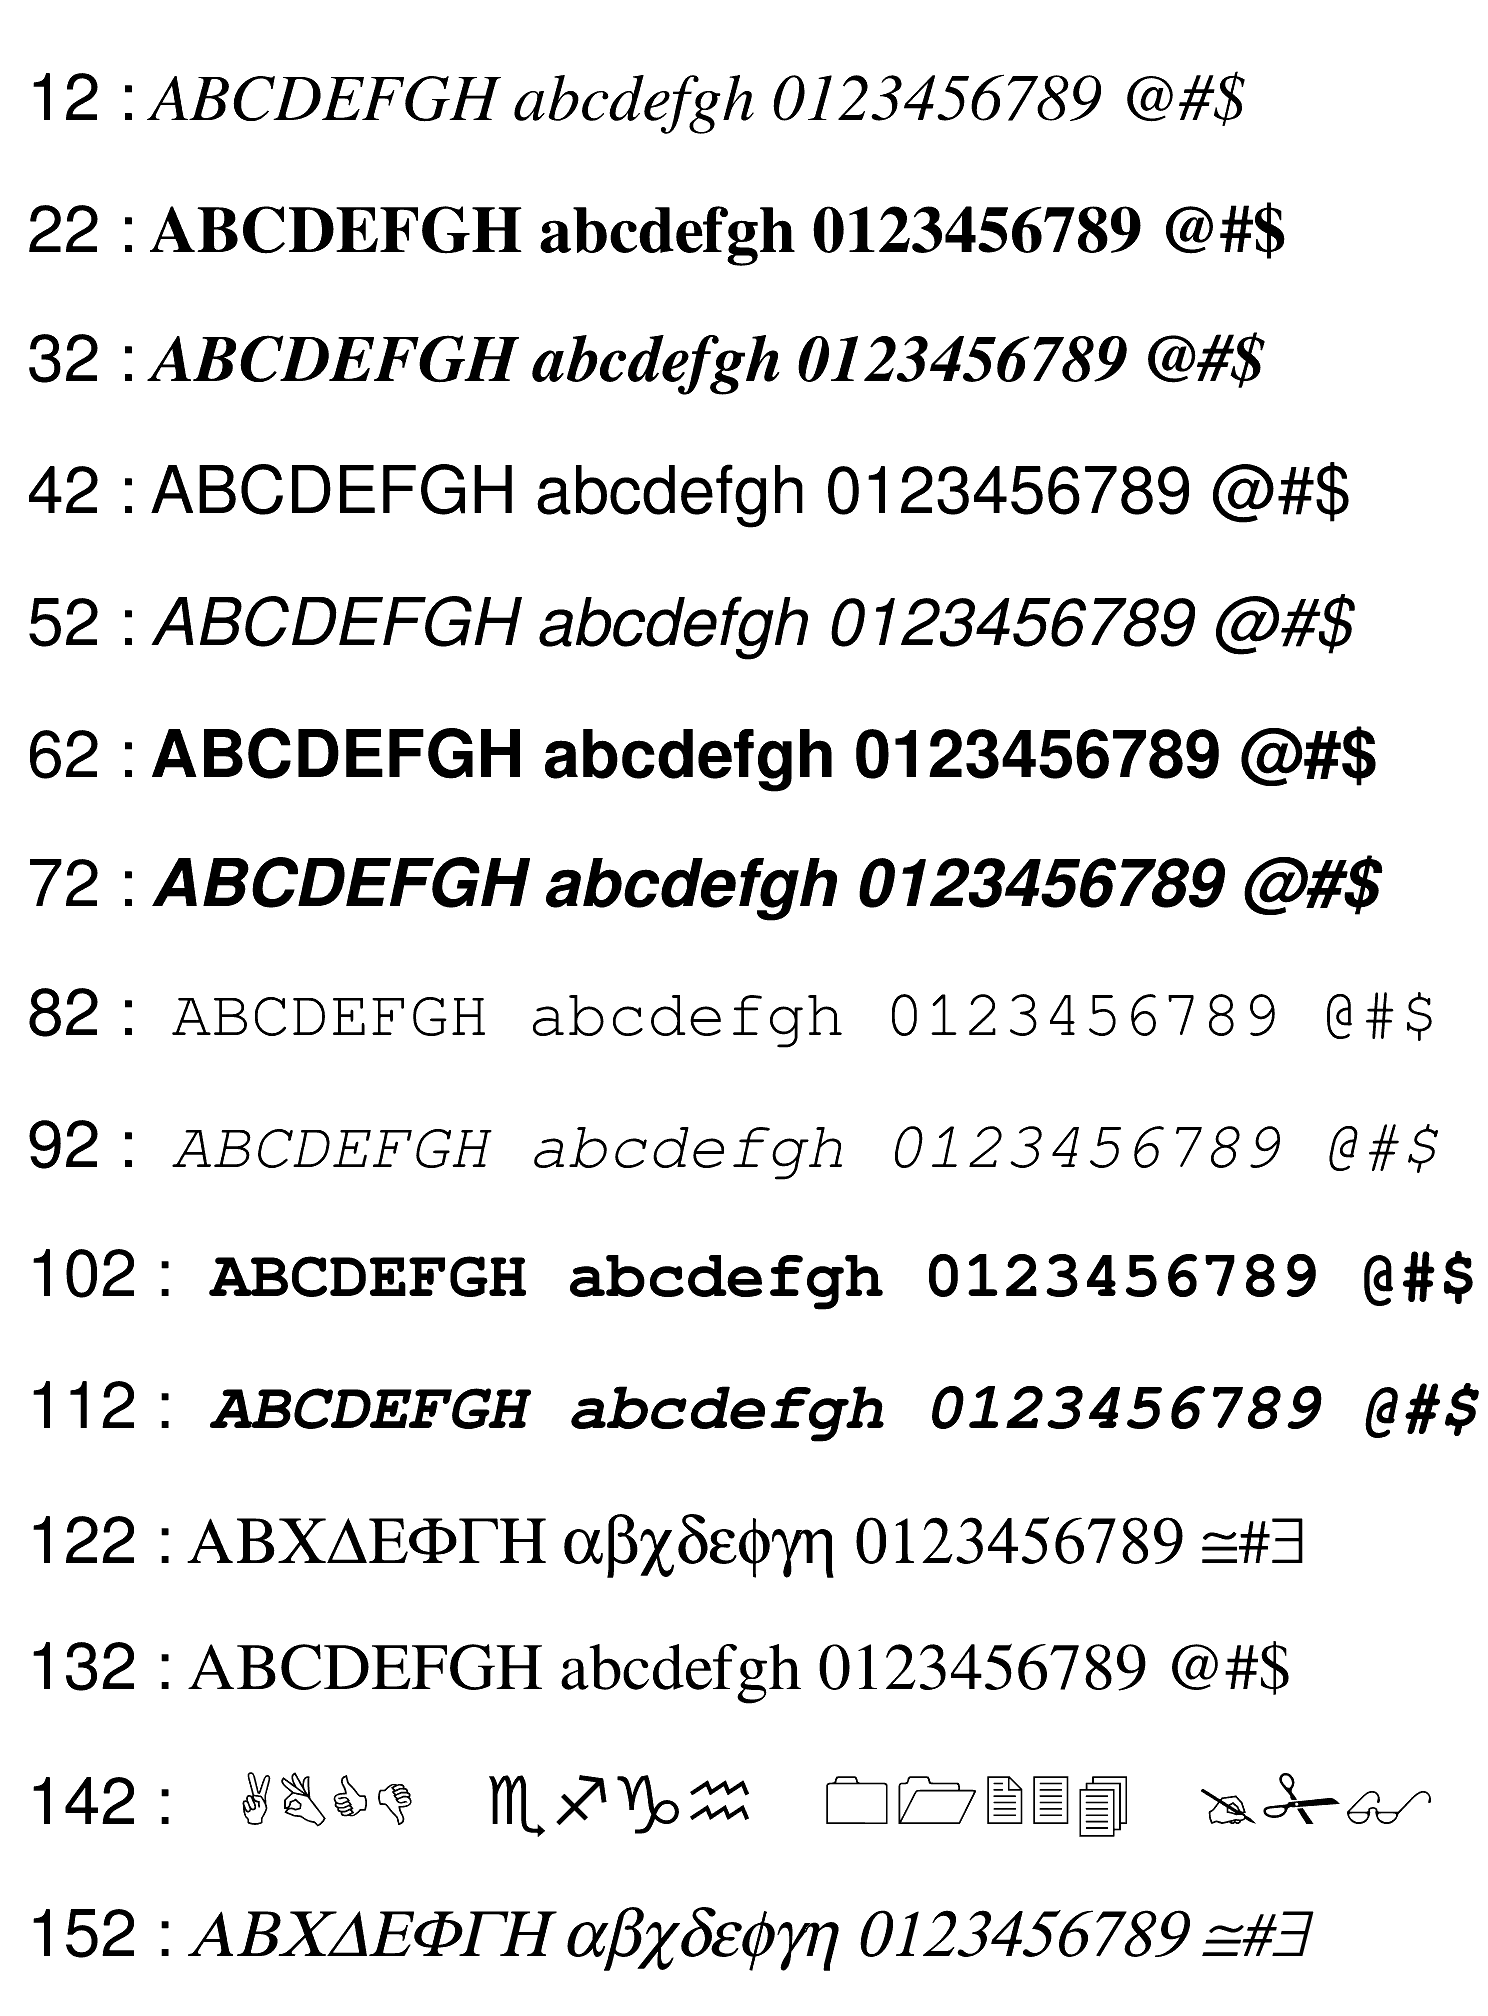
\includegraphics[scale=0.15]{fonts.png}
\end{figure}

\section{Canvas syntax}
\begin{description}
\item[\texttt{TCanvas* myCanvas = new TCanvas()}]
\item[\texttt{TCanvas* myCanvas = new TCanvas()}]
\item[\texttt{myCanvas->Print("<file-name>.<extension>", "<option>")}] prints canvas to file. Possible formats: \texttt{.ps} (Postscript, default one) with options \texttt{Portrait} or \texttt{Landscape}, \texttt{.eps} (encapsulate Postscript), \texttt{.pdf} with option \texttt{Title: <title>}, \texttt{.svg, .tex, .gif, .gif+<N>} (animated gif, where \texttt{N} is the delay in units of 10ms), \texttt{.xpm, .png, .jpg, .tiff, .cxx, .xml, .json, .root}.
\item[\texttt{myCanvas->SetCanvasSize(<x\_px>,<y\_px>)}]
\item[\texttt{myCanvas->SetWindowSize(<x\_px>,<y\_px>}]{}\,\\
If canvas size exceeds window size, scrollbars are displayed
\item[\texttt{myCanvas->GetWh}] get value of window height
\item[\texttt{myCanvas->GetWw}] get value of window width
\item[\texttt{myCanvas->ToggleToolBar()}] hides if shown or vice versa
\end{description}
\subsection*{Pads}
\begin{description}
\item[\texttt{myCanvas->Divide(<nx>, <ny>)}] divides equally into nx$\times$ny pads 
\item[\texttt{myCanvas->Divide(<nx>, <ny>, <x\_margin>, <y\_margin>, <color>)}] Same; margins are given as \textbf{percent of canvas}. \texttt{color} is the color of new pads; 
\end{description}
Pads can be divided in sub-pads.
\begin{description}
\item[\texttt{myCanvas->cd(<pad\_num>)}] sets current pad. Starts from \texttt{1}, \texttt{0} is parent pad (frame). Current pad can be retrieved through \texttt{gPad}. It goes by rows, so the numbering looks like:
\end{description}
\[\begin{bmatrix}
1 & \rightarrow &  n \\
n+1 & \rightarrow & 2n \\
\vdots & \vdots & \vdots\\
(m-1)n + 1 & \rightarrow & mn
\end{bmatrix}\]

\section{Pseudo-Random number generation: TRandom}
Classes with algorithms employed:
\begin{itemize}
\item \texttt{TRandom \, \dotfill \, Linear Congruential Generator}
\begin{center}
\boxed{\textit{ $\nwarrow$ It's a \textbf{very bad} generator, not to be used!}}
\end{center}
\item \texttt{TRandom1 \, \dotfill \, RANLUX}
\item \texttt{TRandom2 \, \dotfill \, Tausworthe}
\item \texttt{TRandom3 \, \dotfill \, Mersenne Twister}
\end{itemize}
\subsection{Methods for generic distributions}
Called on global pointer \texttt{gRandom} or on \texttt{TRandom*} pointer after declaration
\begin{description}
\item[\texttt{Uniform(<double\_1>, <double\_2>)}] uniform distribution on \texttt{\big]double\_1, double\_2\big[} based on \texttt{Rndm()}
\item[\texttt{Rndm()}] uniform in 
\item[\texttt{Uniform(<double>)}] uniform distribution on \texttt{\big]0, double\big[}
\item[\texttt{Integer(<int\_max>)}] uniform \textbf{integer} distribution on \texttt{\big[0, int\_max - 1\big]}
\item[\texttt{Gaus(<mean>, <sigma>)}] (careful, just one '\texttt{s}')
\item[\texttt{Poisson(<mean>)}] \textbf{integer} poissonian distribution
\item[\texttt{PoissonD(<mean>)}] \textbf{double} poissonian distribution
\item[\texttt{Binomial(<n\_tot>, <prob\_of\_succ>)}]
\item[\texttt{Exp(<tau>)}]
\item[\texttt{Landau(<mpv>, <sigma>)}] Landau distribution: \texttt{mpv} is the \textit{most probable value} (moda) and sigma is \textit{not} the SD (which is undefined)
\end{description}

\subsection{Random generation from a generic function}
\begin{verbatim}
TF1 *f1 = new TF1("f1", "<expression>", <xmin>, <xmax>);
double rd = f1->GetRandom();
\end{verbatim}
\texttt{r} is now a random variable distributed according to the PDF defined by \texttt{f1}. It is not necessary to manually ensure that \texttt{f1} is normalized: \textbf{normalization is carried out automatically}, the only requirement on the function is \textbf{continuity}.
\begin{description}
\item[\texttt{histo->FillRandom("<function>", <n>)}] fills the histogram with \texttt{n} extractions from a random variable distributed according to \texttt{f1} (name). Same considerations as before apply.
\end{description}
\subsection{Filling an histo with randomly generated values}
\begin{verbatim}
for(Int_t j=0;j<ngen;j++){ // generation loop
   Double_t x = gRandom->Uniform(xmin,xmax); // extraction
   h->Fill(x); // filling
}
\end{verbatim}

\end{document}
